\documentclass[10pt,conference,compsocconf]{IEEEtran}

\usepackage{hyperref}
\usepackage{graphicx}	% For figure environment


% Umlaute unter UTF8 nutzen
\usepackage[utf8]{inputenc}



% Variablen


% weitere Pakete
% Grafiken aus PNG Dateien einbinden
\usepackage{graphicx}
\usepackage[singlespacing]{setspace}
\usepackage{subcaption}
\usepackage{float}

% Eurozeichen einbinden
\usepackage[right]{eurosym}

% Zeichenencoding
\usepackage[T1]{fontenc}

\usepackage{lmodern}

% floatende Bilder ermöglichen
%\usepackage{floatflt}
\usepackage{tikz}
% mehrseitige Tabellen ermöglichen
\usepackage{longtable}

% Unterstützung für Schriftarten
\newcommand{\changefont}[3]{ 
	\fontfamily{#1} \fontseries{#2} \fontshape{#3} \selectfont}



% Paket für Boxen im Text
\usepackage{fancybox}

\begin{document}
\title{Machine Learning - Project \\ Road Segmentation}

\author{
	Marion Chabrier, Valentin Margraf, Octavianus Sinaga\\
	\textit{Department of Computer Science, EPFL Lausanne, Switzerland}
}

\maketitle

\begin{abstract}
	The goal of this project is to implement and train a Neural Network that is able to segment satellite images into roads and background. We implemented a Convolutional Neural Network and used the Sliding Window Approach in order to tackle this classification task. TO BE ADDED: RESULTS 
\end{abstract}

\section{Introduction}
Image segmentation is a well known task in the field of Deep Learning which can be handled by Neural Networks. There exist different approaches such as Convolutional Neural Networks (\cite{pixelwise}) or newer ones such as the U-Net (\cite{unet}) which both yield good results according to our research.

We decided to choose the Convolutional Neural Network since it seemed very natural to us to classify pixels of the image by taken into account their context inside the image. 
\\\\TO BE ADDEDIn the first section we describe our methods i.e. data augmentation, our model, training of the model as well as tuning of the hyperparameters.
We then present our results obtained with the CNN. Then Discussion..Then Summary.


\section{Methods}
\subsection{Classification Task}
Our Neural Net takes as input parts of the image of size 72x72, so called windows, and classifies if the 16x16 patch in the center of this window belongs to "road" or not. If the net classifies the patch as road, the output should be [1,0]. Hence it will be white in the predicted label.  Otherwise it should be [0,1] and the patch in the label will be black. This is illustrated in Figure 1.
\begin{figure}[htbp]
	\centering
	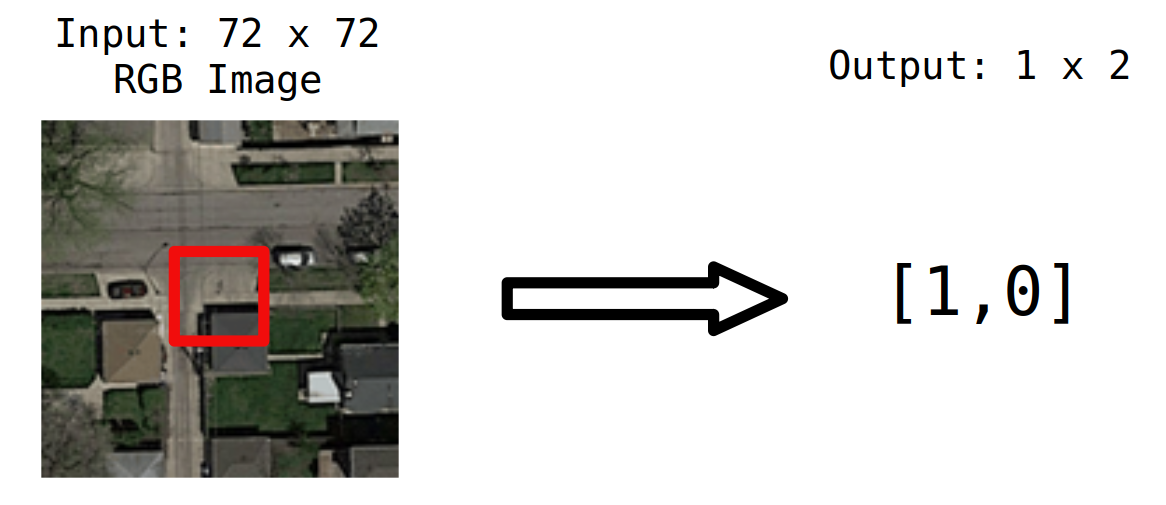
\includegraphics[width=6cm]{images/classificationTask.png}
	\caption{Our CNN classifies if the patch in the center of the window belongs to road or background.}
	\vspace{-3mm}
	\label{fig:clas}
\end{figure}

The idea behind this approach is, that the patch in the center is classified by taken into consideration the surrounding of this patch. E.g. if we have a lot of vehicles near or in the patch, it is more likely that the patch belongs to road. The patch hence is somehow classified by its context in the image. \\


\subsection{Data Augmentation}

The training data consists of 100 RGB satellite images of size 400x400 and their groundtruth (400x400 binary image) respectively. 
Obviously this task is not easy. Sometimes the roads are hidden by a tree or cars may drive on them. 
We therefore augment our training data in order to achieve better results. We rotate each image and its groundtruth by 15, 30, 45, 60, 90, 100, 180 and 270 degrees. When rotating we obtain bigger images, where several parts are just black. We therefore fill those parts by reflecting the image along its boundary axis. Then we crop out images of size 400x400 to get training images and groundtruths in the same size as the 'original' training images, groundtruths respectively.

%
%\begin{figure}[htbp]
%	\centering
%	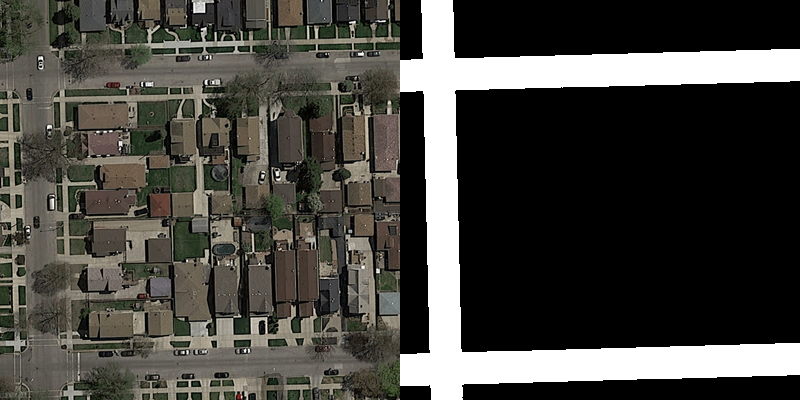
\includegraphics[width=4cm]{images/data_augment.png}
%	\caption{'Original' training image and groundtruth.}
%	\label{fig:dat}
%\end{figure}
%\begin{figure}[htbp]
%	\centering
%	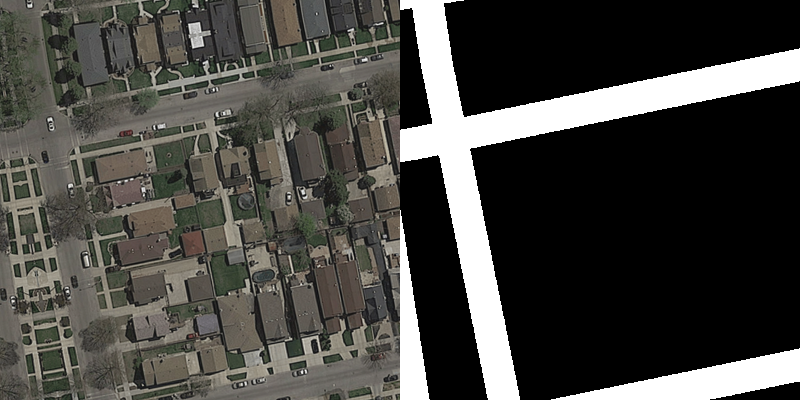
\includegraphics[width=4cm]{images/data_augment_rot.png}
%	\caption{By 15 degrees rotated, reflected along boundary axes and cropped image and groundtruth.}
%	\label{fig:datrot}
%\end{figure}



\begin{figure}[H]
	\centering
	\begin{subfigure}[htb]{0.2\textwidth}
		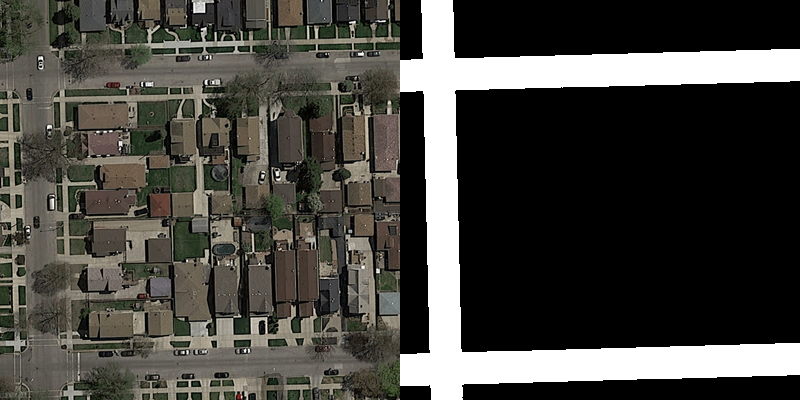
\includegraphics[width=4.2cm]{images/data_augment.png}
		\caption{'Original' training image and label.}
		\label{fig:dat}
	\end{subfigure}
	\hspace{1.5em}
	\begin{subfigure}[htb]{0.2\textwidth}
		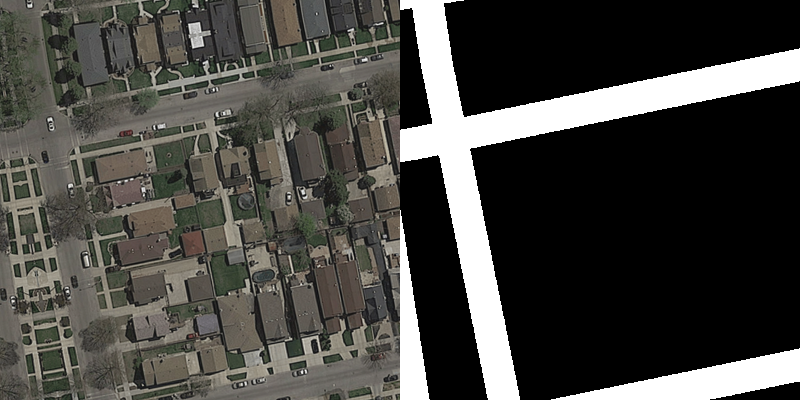
\includegraphics[width=4.2cm]{images/data_augment_rot.png}
		\caption{Rotated training image and label.}
		\label{fig:datrot}
	\end{subfigure}
	\caption{Example of augmenting data: Rotated by 15 degrees, mirrored along the boundary axes and cropped out 400 x 400 pixels.}
\end{figure}

By doing so we augmented the number data by a factor of 9.



\subsection{Convolutional Neural Net}
\label{cnn}
With aim of classifying the whole image we move our window through the whole image. This so called 'sliding window' approach is illustrated in Figure 3.


\begin{figure}[htbp]
	\centering
	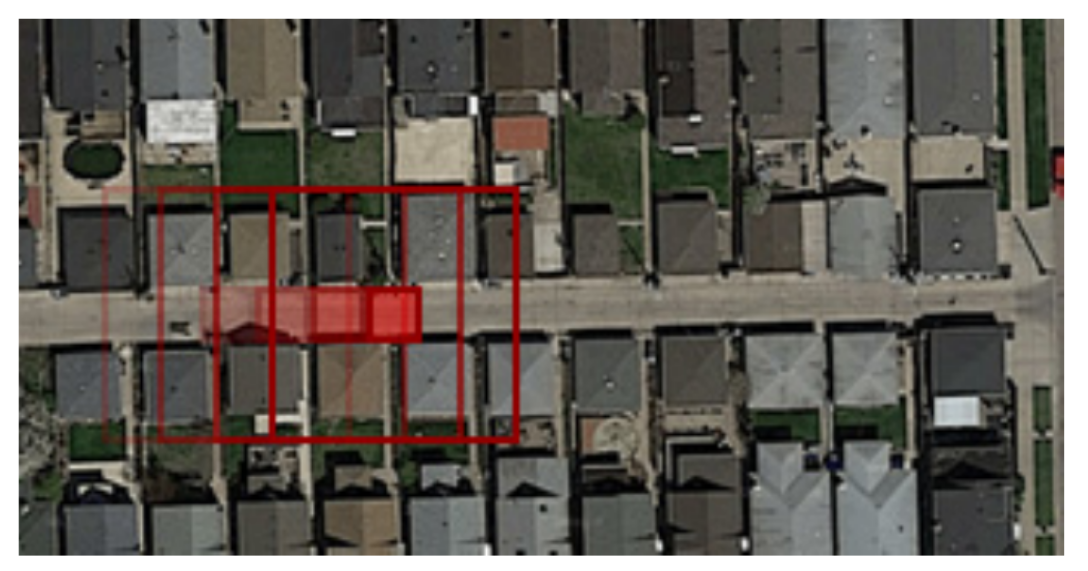
\includegraphics[width=8cm]{images/slidingwindow.png}
	\caption{For each window the patch in the center will be classified. We then move the window through the image by a certain stride.}
	\vspace{-3mm}
	\label{fig:slidwindo}
\end{figure}

In order to apply this technique to patches near the border, we have to somehow enlarge the images. We therefore choose a padding method: At the border we reflect each image along its boundary axes.
\\
The architecture of our Convolutional Neural Net is displayed in Table 1. 
TO BE ADDED CHOICE OF LAYERS, DROPOUT

\begin{table}[htbp]
	\centering
	\begin{tabular}[c]{|l||l|}
		\hline
		\textbf{Layer}&\textbf{Characteristics}\\
		\hline
		Input&72x72x3 RGB\\
		Conv + LReLU &64 filter each 5x5\\
		Max Pooling&2x2\\		
		Dropout&0.25\\
		\hline
		Conv + LReLU &128 filter each 3x3\\
		Max Pool&2x2\\		
		Dropout&0.25\\
		\hline
		Conv + LReLU &256 filter each 3x3\\
		Max Pool&2x2\\		
		Dropout&0.25\\
		\hline
		Dense + LReLU &128 nodes\\
		Dropout&0.5\\		
		Softmax + Output&2 labels\\
		\hline
	\end{tabular}
	\caption{Architecture of the Convolutional Neural Network.}
	\label{tab:cnn_architecture}
\end{table}



\subsection{Training}

In the training process we randomly choose a window of an image of the training data. We then compute the corresponding patch of the groundtruth image. The groundtruth label is then given by the mean of all pixels in this patch: If it is higher than a certain threshold, 0.25 in our case, then the label will be black, otherwise white.\\
By doing so we get even much more training data since each window of each image corresponds to one training image. But since some of the windows overlap themselves, we don't gain much more information by using all of them.


TO BE ADDED. TUNED HYPERPARAMETERS: ALPHA, DROPOUT, ACTIVATION FUNCTIONS , WINDOW/PATCH SIZE!"!! WHY WE CHOSE THEM IN THIS MANNER
takes a lot of tim 3 000 000 parameters to be trained
GPU BLABLA




\subsection{Prediction}

The test image data consists of 50 RGB satellite images of size 608x608. We first have to some data preparation: We enlarge the images by a padding method similar the one explained in section \ref{cnn}. After cropping the image into windows of size 72x72, we feed each patch of each window into our neural network and predict a label for it. We get our final predictions by mapping each labels back to its corresponding patch and setting these patches together to an image.


for each window predict label for the patch in the center. stride = patch.size
gives us 1444 labels, because 608x608 contains 1444 16x16 patches. we then finally convert the labels to images..

\begin{figure}[H]
	\centering
	\begin{subfigure}[htb]{0.2\textwidth}
		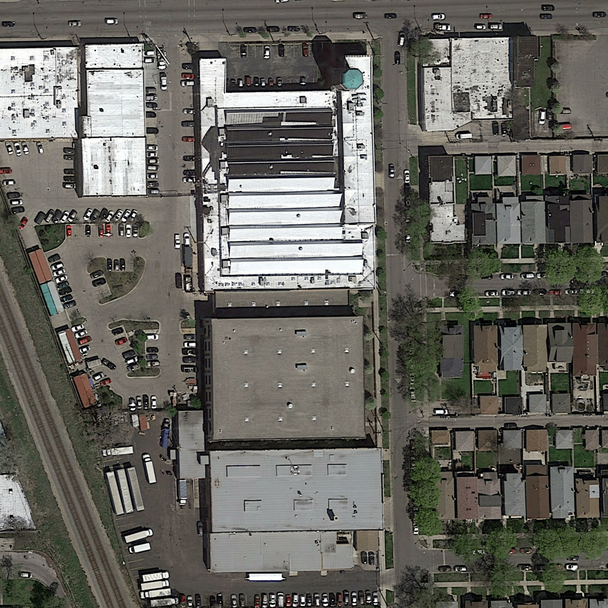
\includegraphics[width=4.2cm]{images/visualize_pred/images/test_2.png}
		\label{fig:test2}
	\end{subfigure}
	\hspace{1.5em}
	\begin{subfigure}[htb]{0.2\textwidth}
		
\includegraphics[width=4.2cm]{images/visualize_pred/groundtruth/pred_2.png}
		\label{fig:pred2}
	\end{subfigure}
	\caption{Test image 2 and its prediction.}
\end{figure}

\begin{figure}[H]
	\centering
	\begin{subfigure}[htb]{0.2\textwidth}
		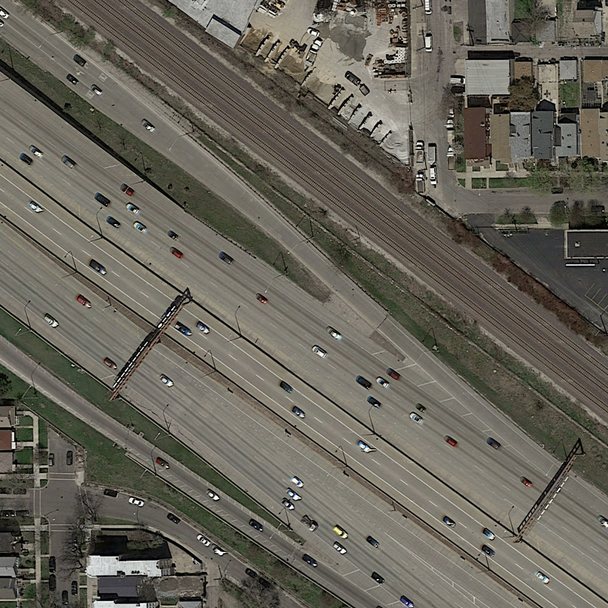
\includegraphics[width=4.2cm]{images/visualize_pred/images/test_9.png}
		\label{fig:test9}
	\end{subfigure}
	\hspace{1.5em}
	\begin{subfigure}[htb]{0.2\textwidth}
		
\includegraphics[width=4.2cm]{images/visualize_pred/groundtruth/pred_9.png}
		\label{fig:pred9}
	\end{subfigure}
	\caption{Test image 9 and its prediction.}
\end{figure}


\section{Results}

images of image and predicted segmentation


\section{Discussion}


As one can oberve, a patch size of 16x16 and window size of 72x72 gives not very smooth predictions of road. This is obviously caused by the fact, that we predict one label for a whole patch. If we choose smaller patches, we would get probably smoother result. But this would also lead to much more computational cost.


\section{Summary}




\section*{Acknowledgements}


\bibliographystyle{IEEEtran}
\bibliography{literature}

\end{document}